\documentclass[11pt]{article}
\usepackage[a4paper,margin=22mm]{geometry}
\usepackage{booktabs,tabularx,array,graphicx,amsmath,xcolor,float,tikz,pgfplots}
\pgfplotsset{compat=1.18}\usepackage[hidelinks]{hyperref}
\setlength{\parskip}{.45em}\setlength{\parindent}{0pt}\emergencystretch=3em
\def\fitlabel{Training-set overall recall}\def\controlname{Control}\def\treatmentname{Treatment}
\def\objectlabel{Interior Dead objects}\def\retained{Retained}\def\gained{Gained}\def\lost{Lost}\def\missed{Missed by both}\def\seedname{Seed}
\def\roundxlabel{Dead hit change: treatment minus same-round control}\def\seedlabel{Seed}
\def\fractionlabel{Fraction}\def\deadlabel{Dead recall}\def\overalllabel{Overall recall}\def\precisionlabel{Precision}
\def\fitdead{Training-set Dead recall}\def\auditdead{Evaluation-set Dead recall}
\title{\bfseries Nucleus-center localization: experiments and object-level diagnosis\\\large Stage report 7}\author{bdd26 research}\date{10 November 2026}\begin{document}\maketitle\tableofcontents\newpage
\section{Question and stage findings}
The model places one center point per nucleus. The development evaluation set contains 522 images and 12,250 nuclei, including 145 interior Dead nuclei in 11 images; the training set contains 2,134 images. One-to-one matching uses a three-pixel radius. Overall recall measures coverage of annotated nuclei, Dead recall measures the annotated Dead subgroup, and precision is the fraction of predicted points that match.

P17 exposed a coverage collapse on training images. P19 halved the number of optimizer updates per epoch and reduced training-set coverage. P20 gained Dead matches at about 4.3 times the training cost. P21's auxiliary semantic head improved training-set performance while evaluation coverage fell. P22 full-depth adaptation produced the strongest consistent Dead gains and fewer extra points. P23 weight averaging changed only a few Dead matches; P24 improved precision with tissue-dependent changes; P25 improved overall point coverage; P26 anchoring reduced overall recall and precision. The following sections trace these outcomes to individual images and nuclei.
\begin{figure}[H]\centering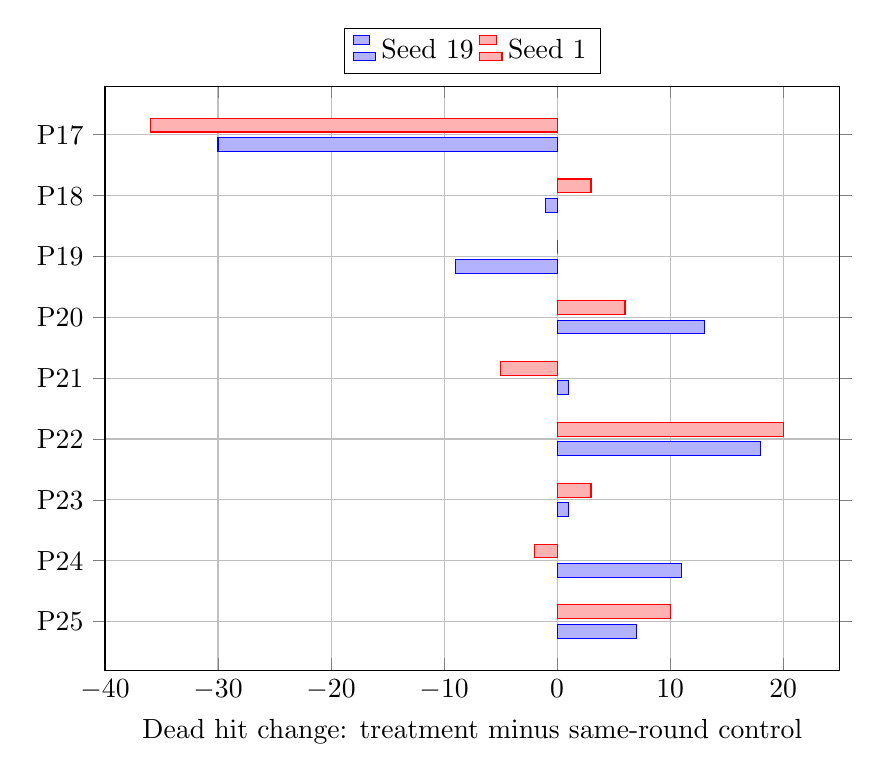
\begin{tikzpicture}
\begin{axis}[xbar, width=.9\linewidth,height=9cm, xmin=-40,xmax=25,
 xlabel={\roundxlabel}, symbolic y coords={P25,P24,P23,P22,P21,P20,P19,P18,P17},
 ytick=data, legend style={at={(.5,1.1)},anchor=north,legend columns=2},
 grid=major,bar width=5pt]
\addplot coordinates { (7,P25) (11,P24) (1,P23) (18,P22) (1,P21) (13,P20) (-9,P19) (-1,P18) (-30,P17) };
\addplot coordinates { (10,P25) (-2,P24) (3,P23) (20,P22) (-5,P21) (6,P20) (0,P19) (3,P18) (-36,P17) };
\legend{\seedlabel\ 19,\seedlabel\ 1}
\end{axis}\end{tikzpicture}
\caption{Dead hit changes within each round and seed, out of 145; P22 shows the largest gain in each seed.}\end{figure}
\section{P17--P21: training, optimization and image scale}
\subsection{P17: high precision from a small set of candidates}
The scratch CNN K produced 1,795 points and matched 1,709 in seed 19, giving 95.21\% precision. Its matched UNI control produced 10,644 points and matched 7,285, giving 68.44\% precision. K emitted no point in 198/522 evaluation images, versus 22 for C. Training-set recall was 14.41\%/11.92\% and evaluation recall 13.95\%/11.89\%; Dead hits were 30/31 versus 60/67 for C. The model produced few predictions, a high proportion of which matched annotations.

\subsection{P18: RGB residual path}
Adding the RGB path H raised seed-19 training-set recall from 97.43\% to 98.52\% and evaluation matches from 7,172 to 7,361. Seed 1 gained 37 evaluation matches. Dead hits changed 71 to 70 and 64 to 67. Seed 19 gained four Dead hits in lung and lost five in colon; seed 1 gained two in each tissue and lost two in cervix. The overall gain and the tissue-specific changes describe different parts of the same result.

\subsection{P19: effective batch and optimizer steps}
Increasing effective batch from 16 to 32 reduced AdamW updates per epoch from 134 to 67. Training-set recall fell from 97.37\% to 94.74\% and from 97.91\% to 94.10\%; Dead hits changed 66 to 57 and 63 to 63. In seed 1 colon gained five, while esophagus and lung lost four and two. The decline in training-set recall appears alongside fewer updates under the fixed 130-epoch schedule. Training time fell by only 1.5--1.9\% with the same physical batch.

\subsection{P20: larger encoder input}
Interpolating the input from 256 to 512 raised Dead hits from 66 to 79 and 69 to 75. Seed 19 gained ten in lung and five in colon, while losing two in cervix. Seed 1 gained four in lung and five in cervix, while losing three in esophagus. Small-Dead hits changed 7 to 9 and 8 to 7. Training-set Dead hits rose from 629/627 to 653/655; evaluation matches changed by +3 and -244. Treatment training took 17.1--17.3 hours versus about 4 hours for C.

\subsection{P21: five-class center supervision}
Auxiliary arm A reduced evaluation matches from 7,300 to 7,132 and 7,389 to 7,241. Dead hits changed 64 to 65 and 70 to 65. In seed 1 an esophagus image fell from 7/8 to 2/8 and a lung image from 11 to 7; small Dead fell from 10/32 to 5/32. Training-set matching rose while evaluation matching fell.

Lung image 1025 contains 38 annotated nuclei including 25 interior Dead. Seed-19 C produced 38 points and matched 29; A produced 39 and matched 27. The green, red and orange marks show the spatial changes in matched, missed and extra points.
\begin{figure}[H]\centering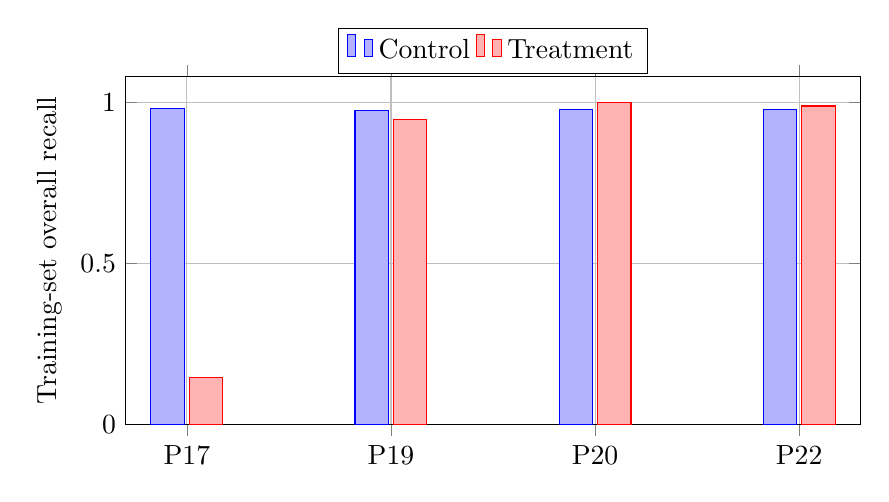
\begin{tikzpicture}
\begin{axis}[ybar,bar width=12pt,width=.9\linewidth,height=6cm,ymin=0,ymax=1.08,
 ylabel={\fitlabel},symbolic x coords={P17,P19,P20,P22},xtick=data,grid=major,
 legend style={at={(.5,1.14)},anchor=north,legend columns=2},point meta=explicit symbolic]
\addplot coordinates {(P17,.9789) [0.979] (P19,.9737) [0.974] (P20,.9785) [0.979] (P22,.9777) [0.978]};
\addplot coordinates {(P17,.1441) [0.144] (P19,.9474) [0.947] (P20,.9976) [0.998] (P22,.9882) [0.988]};
\legend{\controlname,\treatmentname}\end{axis}\end{tikzpicture}\caption{Seed-19 training-set recall for each round’s control and treatment.}\end{figure}
\begin{figure}[H]\centering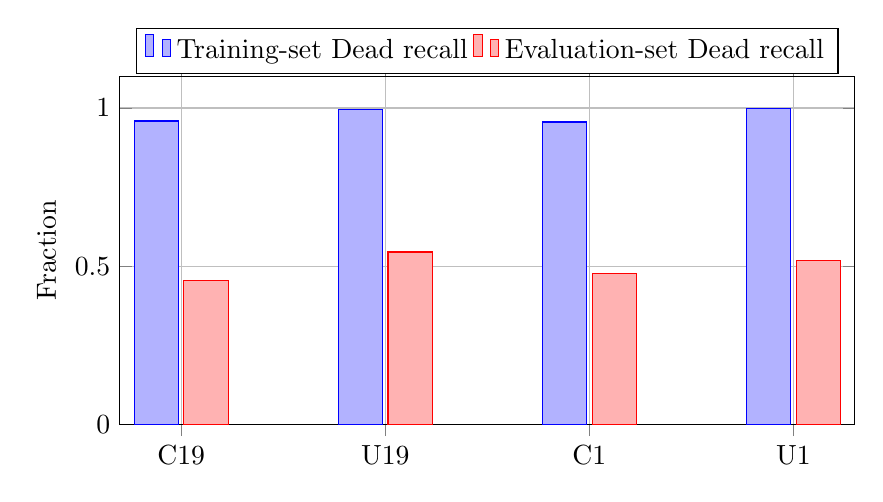
\begin{tikzpicture}
\begin{axis}[ybar,bar width=16pt,width=.9\linewidth,height=6cm,ymin=0,ymax=1.1,
 ylabel={\fractionlabel},symbolic x coords={C19,U19,C1,U1},xtick=data,grid=major,
 legend style={at={(.5,1.14)},anchor=north,legend columns=2}]
\addplot coordinates {(C19,.95884) (U19,.99543) (C1,.95579) (U1,.99848)};
\addplot coordinates {(C19,.45517) (U19,.54483) (C1,.47586) (U1,.51724)};
\legend{\fitdead,\auditdead}\end{axis}\end{tikzpicture}\caption{P20 Dead recall on training and evaluation images; C encodes 256 pixels, U encodes an interpolated 512-pixel image.}\end{figure}
\begin{figure}[H]\centering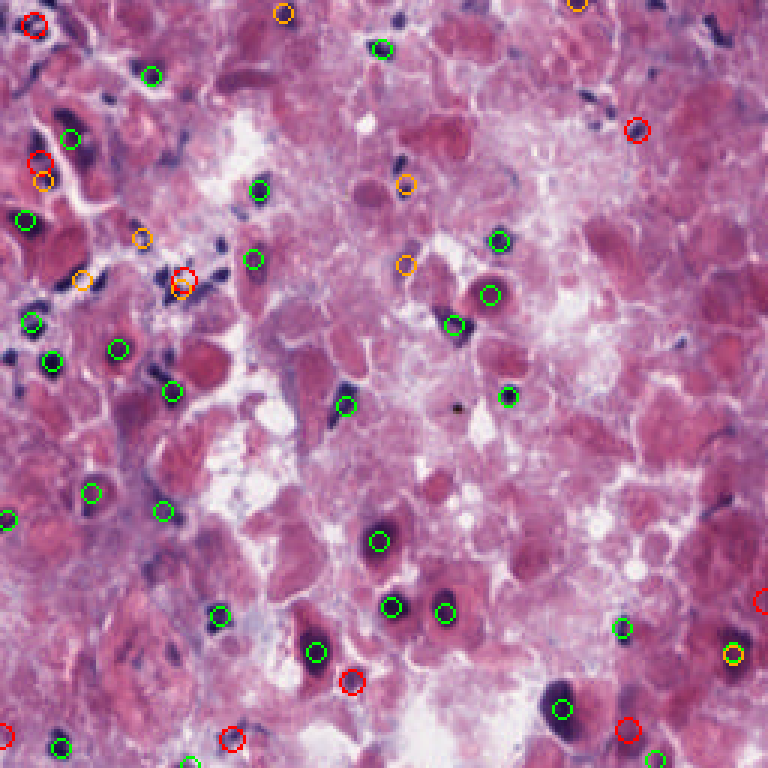
\includegraphics[width=.47\linewidth]{assets/casebook/p21_c_1025.png}\hfill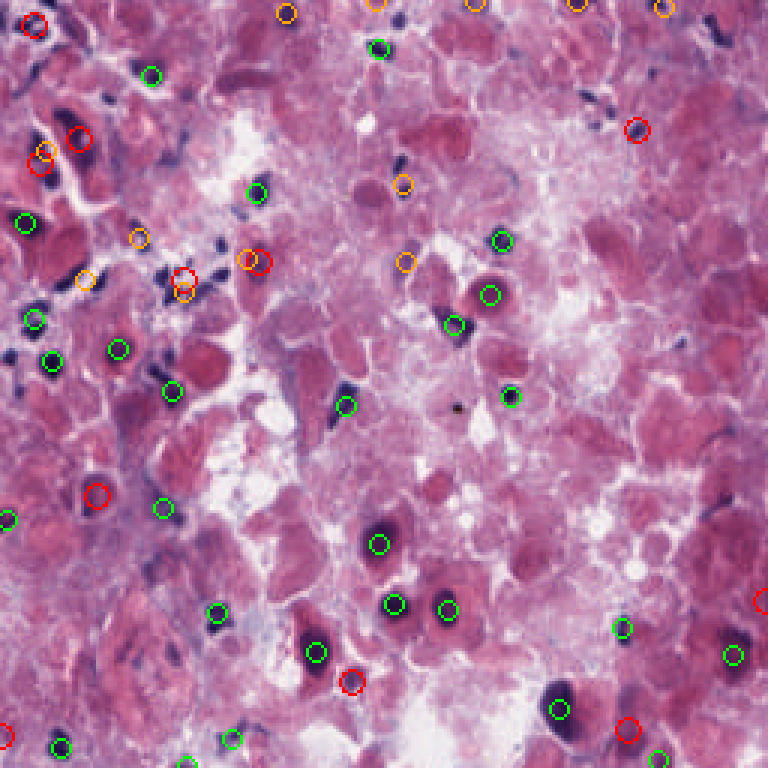
\includegraphics[width=.47\linewidth]{assets/casebook/p21_a_1025.png}\caption{P21 lung image 1025: C left, A right. Green: matched; red: missed; orange: extra.}\end{figure}
\section{P22: which nuclei did full-depth adaptation recover?}
Control C adapts the last 12 UNI blocks and M adapts all 24. Dead hits rose 67 to 85 and 62 to 82; overall recall rose 6.02 and 6.15 percentage points, and precision 3.64 and 3.46 points. Seed 19 produced 488 more candidates and 738 more matches, reducing extra points by 250. Seed 1 produced 542 more candidates and 753 more matches, reducing extra points by 211. Training time increased by 42--43\%, with peak memory rising from 4.05 to 6.75 GiB.

Of 145 Dead objects, seed 19 retained 55 hits, gained 30, lost 12 and missed 48 in both arms; seed 1 retained 56, gained 26, lost 6 and missed 57 in both. Seed-19 lung contributed a net 12 and cervix a net 7. Colon had five gains and five losses. Small-Dead hits rose from 7/32 to 11/32 in both seeds.

Each crop below shows the original image, C matching and M matching. The white-and-black ring marks the same annotated nucleus. Green marks a match, red a miss and orange an extra point. Each 80-by-80-pixel crop is enlarged by nearest-neighbor interpolation. The reported score is the maximum value in the center-prediction map within three pixels of the annotated center. The fixed score threshold is 0.5, followed by peak selection and one-to-one matching.
\begin{figure}[H]\centering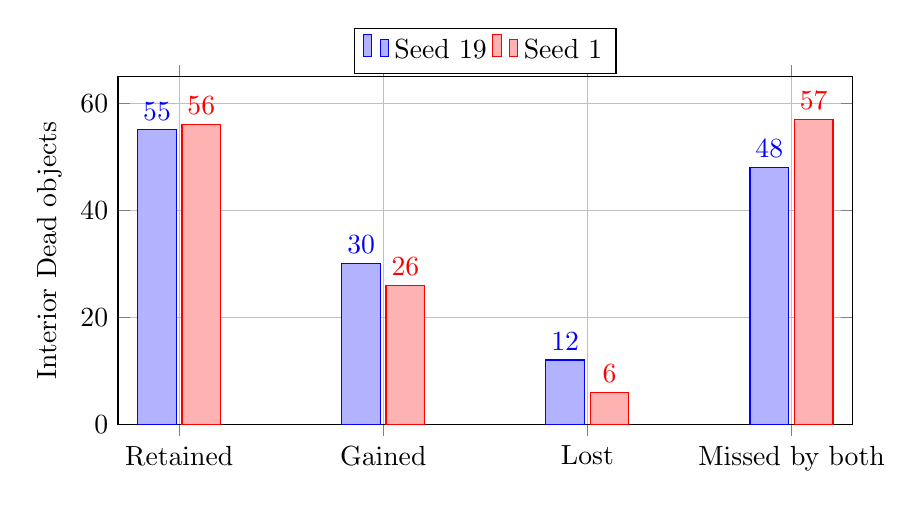
\begin{tikzpicture}
\begin{axis}[ybar,bar width=14pt,width=.9\linewidth,height=6cm,ymin=0,ymax=65,
 ylabel={\objectlabel},symbolic x coords={Retained,Gained,Lost,Missed},xtick=data,
 xticklabels={\retained,\gained,\lost,\missed},grid=major,nodes near coords,
 legend style={at={(.5,1.14)},anchor=north,legend columns=2}]
\addplot coordinates {(Retained,55) (Gained,30) (Lost,12) (Missed,48)};
\addplot coordinates {(Retained,56) (Gained,26) (Lost,6) (Missed,57)};
\legend{\seedname\ 19,\seedname\ 1}\end{axis}\end{tikzpicture}\caption{P22 object-level transitions, totaling 145 for each seed.}\end{figure}
\begin{figure}[H]\centering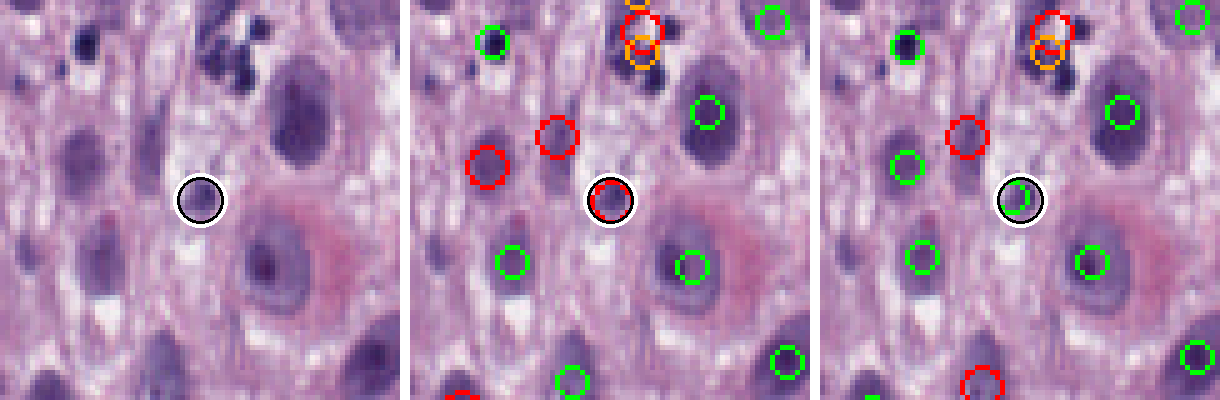
\includegraphics[width=.98\linewidth]{assets/casebook/recovered_1037.png}\caption{Lung 1037, object 67 (row 98, column 180; area 65 pixels): C response approximately 0, M 0.792; miss becomes match.}\end{figure}
The small nucleus lies beside darker staining. C gives a red miss at this location; M gives a green match.
\begin{figure}[H]\centering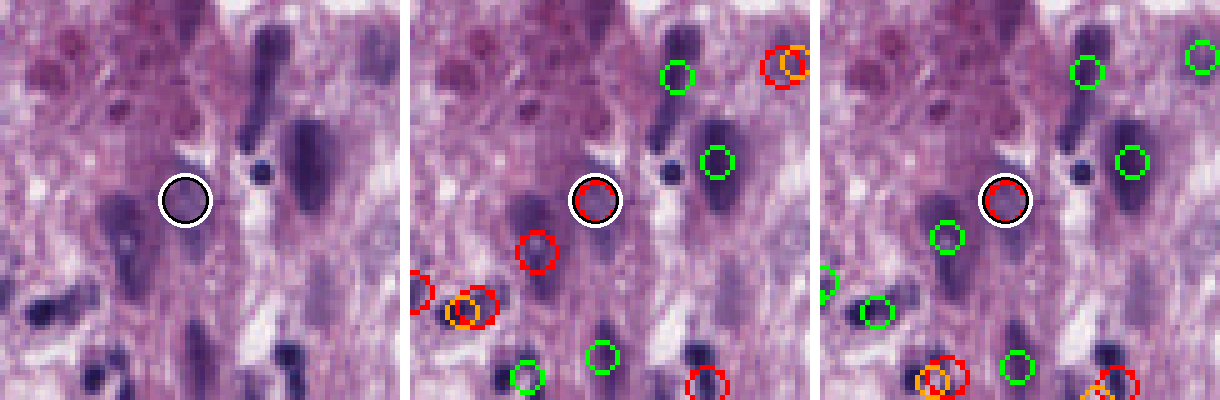
\includegraphics[width=.98\linewidth]{assets/casebook/missed_1037.png}\caption{Lung 1037, object 57 (row 43, column 37; area 214 pixels): C response approximately 0, M 0.446; both outputs miss it.}\end{figure}
The nucleus lies among several dark-stained structures. M increases the response but it remains below 0.5, leaving a red miss.
\begin{figure}[H]\centering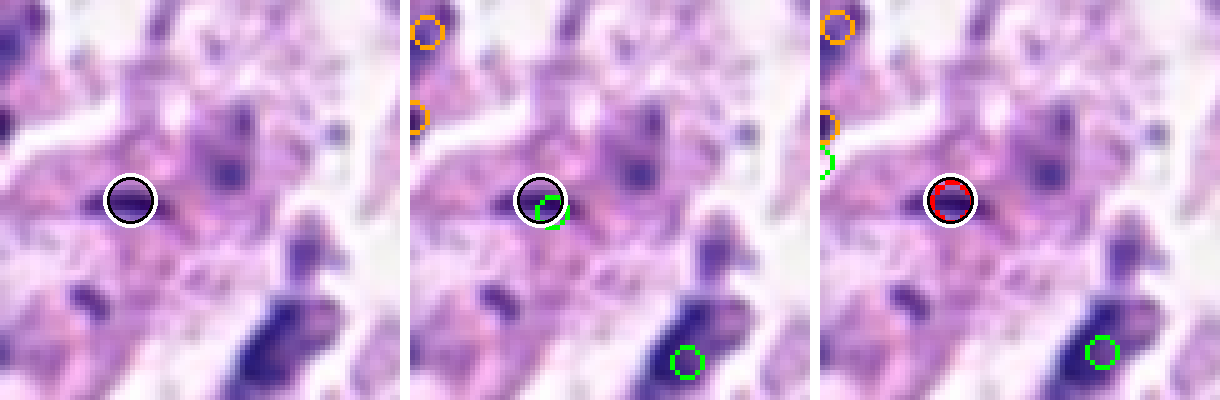
\includegraphics[width=.98\linewidth]{assets/casebook/lost_0776.png}\caption{Colon 776, object 7 (row 148, column 26; area 137 pixels): C response 0.835 and matched; M response 0.146 and missed.}\end{figure}
The same annotated position changes from green to red. The object-level record reveals exchanges that net counts compress.
\section{P23--P26: averaging, learning rates and anchoring}
\subsection{P23: Moving-average parameters preserve most existing detections}
Each seed produces final C and exponential-moving-average E weights from one trajectory. Dead hits changed 69 to 70 and 60 to 63; small Dead remained 6/32 in all four outputs. In seed 19 all 69 existing matches were retained, one low-response object became matched, and 72 remained low-response. The seed-19 gain was in lung image 1025; seed-1 gains occurred in colon 776, colon 1482 and cervix 1756.

\subsection{P24: higher learning rate improves precision unevenly across images}
Increasing the last-12 learning rate from $10^{-5}$ to $3\times10^{-5}$ raised precision from 0.688 to 0.732 and 0.694 to 0.731. Candidate counts fell by 589/471 while all-nucleus matches rose by 29/38. Dead hits changed 67 to 78 and 68 to 66. Small-Dead hits rose 7/32 to 11/32 in both seeds; changes among larger Dead were +7 and -6. Lung image 1037 gained 5/3 Dead hits, whereas lung 1025 lost 1/3; cervix 1756 changed +2/-4. In the image below several red marks turn green in L, while other red and orange marks remain.

\begin{figure}[H]\centering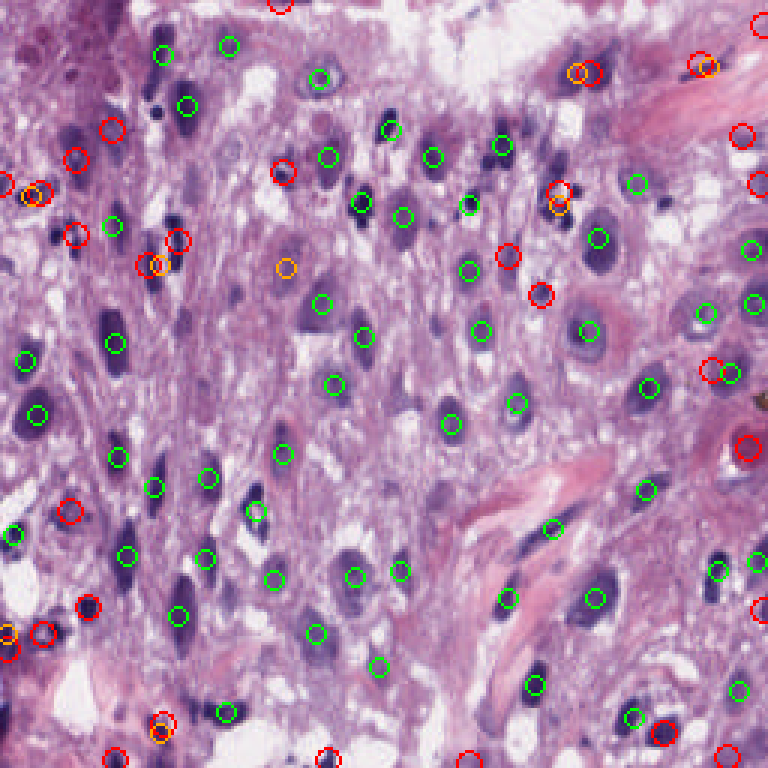
\includegraphics[width=.47\linewidth]{assets/casebook/p24_c_1037.png}\hfill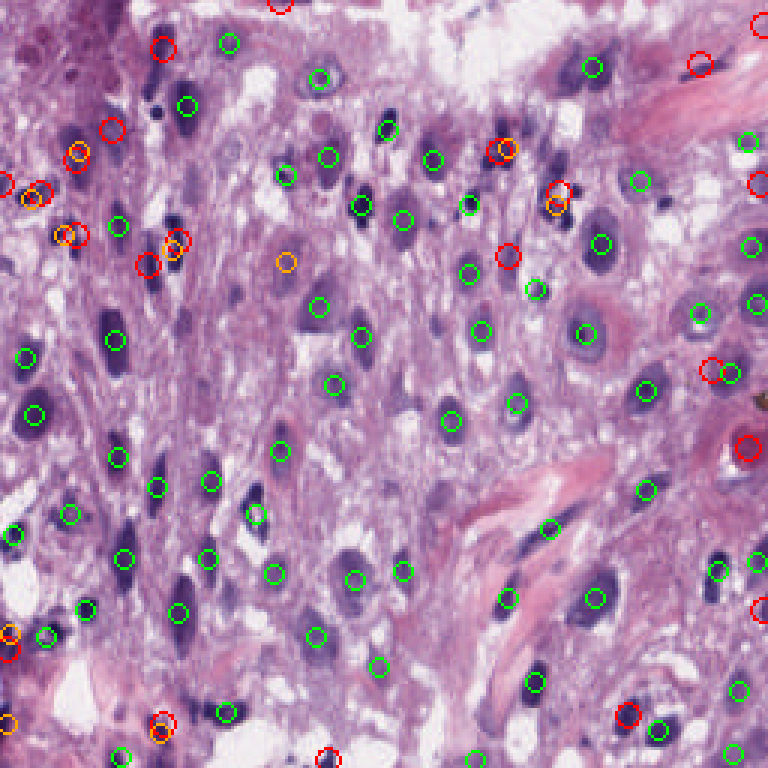
\includegraphics[width=.47\linewidth]{assets/casebook/p24_l_1037.png}\caption{P24 lung image 1037, seed 19: C left, L right. Green marks matches, red misses, orange extras.}\end{figure}
\subsection{P25: layerwise adaptation across all blocks}
The 24-block layerwise recipe raised overall recall from 0.590/0.598 to 0.650/0.640 and precision from 0.690/0.692 to 0.744/0.742. Dead hits changed 69 to 76 and 65 to 75. Matches increased by 741/512 while extra points fell by 510/544. Lung image 1037 changed 10 to 15 and 10 to 16; colon image 1482 changed 15 to 9 and 14 to 10. The lung and colon changes move in opposite directions and partially offset each other in both seeds.

\subsection{P26: anchoring to pretrained weights}
All four tasks completed 130 epochs. Dead hits changed 67 to 69 and 64 to 66. R overall recall was 0.571/0.569 versus C 0.584/0.596; R precision was 0.679/0.688 versus C 0.697/0.693. Both paired Dead gains were 2/145, with original intervals $[-0.006173,0.053793]$ and $[-0.071429,0.061224]$. The anchor reduced overall coverage and precision in this comparison, with a small Dead change.

\section{Synthesis: where misses arise}
Across the four P22 models, 94.87\%--97.59\% of missed Dead objects had a maximum center-prediction score below 0.5 within three pixels of the annotated center. Seed-19 C/M had 74/57 such low-response objects and 4/3 misses associated with localization or suppression of nearby duplicate predictions. Object 57 illustrates a response that rises yet remains below threshold; object 67 crosses the threshold and matches; colon object 7 shows a response that weakens in the same comparison. These locations guide further inspection of local features, similar nuclei in the training set and center-response distributions across tissues.

Pairwise results use each round's own same-seed control. \texttt{NUMBER\_SOURCES.md} records source files, matching definitions and image provenance.
\begin{figure}[H]\centering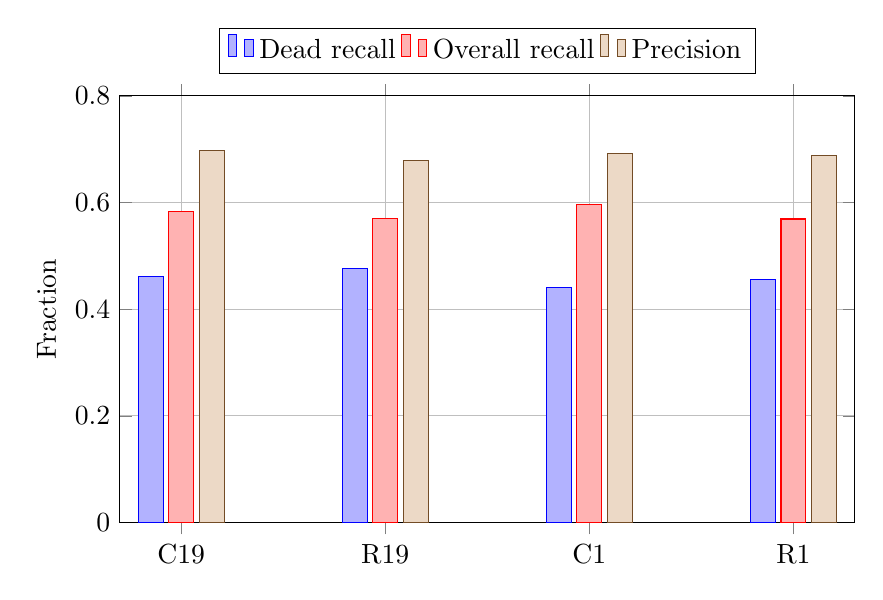
\begin{tikzpicture}
\begin{axis}[ybar,bar width=9pt,width=.90\linewidth,height=7cm,ymin=0,ymax=.8,
 ylabel={\fractionlabel},symbolic x coords={C19,R19,C1,R1},xtick=data,grid=major,
 legend style={at={(.5,1.16)},anchor=north,legend columns=3}]
\addplot coordinates {(C19,.462069) (R19,.475862) (C1,.441379) (R1,.455172)};
\addplot coordinates {(C19,.583673) (R19,.570857) (C1,.596245) (R1,.569224)};
\addplot coordinates {(C19,.697221) (R19,.678537) (C1,.692519) (R1,.688080)};
\legend{\deadlabel,\overalllabel,\precisionlabel}
\end{axis}\end{tikzpicture}
\caption{P26 evaluation metrics for C and R in both seeds.}\end{figure}
\end{document}
